\documentclass{article}
\usepackage[GBK]{ctex}
\usepackage{booktabs} % 用于表格
\usepackage{longtable} % 用于长表格
\usepackage{geometry} % 控制页面边距
\usepackage{color}
\usepackage{type1cm} 
\usepackage{graphicx} % 图片
\geometry{a4paper, margin=1.1in}

\title{
HKU-MSc Computer Science
Admission Test Compilation
}
\author{Weicong HUANG, stalwarthuang@outlook.com}
\date{December 2024}

\begin{document}

% \setlength{\parindent}{0pt} % 禁用段落缩进


\maketitle


\vspace{-3.5em} % 调整声明与标题之间的间距
\begin{center}
\textit{The following questions represent a selection from the entrance examination for the MSc in Computer Science at The University of Hong Kong. 
They have been sourced from online and are intended for personal study, research and communication purposes only!.}
\end{center}
\vspace{2em} 

\section{Programming}

\noindent\textbf{(20 marks)} A positive integer \(n > 2\) is sacred if \(n = a^2 + b^3\) for some integers \(a\) and \(b\). Write a program (using either the programming language C, C++, Java, Python) that repeatedly asks the user to input a positive integer \(n\), and prints "YES" if it is sacred, and "NO" otherwise. The program stops if a negative integer is input.

\vspace{2\baselineskip} % 空两行

\noindent\textbf{(10 marks)} There are 150 cards, each with a different number written on it.The cards are arranged in a 15 x 10 grid such that each row is arranged in increasing order from left to right, and each column is arranged in increasing order from top to bottom. All cards are face down, making it impossible to see the numbers on them. Your task is to find a specific number $x$. You need to design a method that will allow you to find the card with number $x$ while turning up as few cards as possible. Additionally, if the number $x$ is not among the 150 cards, your method should be able to determine this. Describe your method in whatever way you feel comfortable (it is okay to use pseudocode or flowchart). What is the minimum number of cards your method will need to turn up in the worst-case scenario? Justify your answer.

\vspace{2\baselineskip}

\noindent Suppose $is\_prime(m)$ is a build-in function that returns "True" if $m$ is a prime number, and returns "False" otherwise.
A positive integer is special if it has two factors $f$ and $f+2$ where both $f$ and $f$ are prime. Write a complete program (in any programming language) that inputs an positive integer $x$, and prints "Yes" if x is special, and "No" otherwise. You may use the function  in your program. (Note: 1 is a factor any any positive integer.)

\vspace{5\baselineskip}


\noindent The following method for finding the square-root of a positive number is known to the ancient Babylonians (1500 BC).

\hangindent=2em % 设置悬挂缩进
\hangafter=1     % 从第二行开始生效
\textit{1.Make an initial guess. Guess any positive number $x_0$.}\\
\textit{2.Improve the guess: Apply the formula $x_1 = (x_0+S/x_0) / 2$. The number $x_1$ is a better estimate to the square root of $S$.}\\
\textit{3.Iterate until convergence: Apply the formula $x_(n+1) = (x_n+S/x_n) / 2$ until the process converges (i.e., the difference between $x_(n+1)-x_n$is smaller than some small numbers.}

\noindent a.(8\%) Apply the above method to find the square-root of $S=20$. Your answer needs to show all the values of $x_0, x_1, ...$\\
\noindent b.(12\%) Write a program (either in C, C++, Java or Python)that implements the above algorithm to find square of a positive, i.e., it asks the user to inputs a positive number $S$, and then prints the square root of $S$.

\vspace{2\baselineskip}

\noindent A bag contains $n$ balls, and the number of balls that can be removed at a time is limited to 1, 2, or 3. Provide a list of all possible scenarios that could result from this process.

\vspace{2\baselineskip}

\noindent A series $a_1, a_2, a_3...a_n$, if satisfied $a_1 < a_2 <a_3 <...< a_i > a_(i+1) > ... > a_n$, is said to be a single-peaked series, if the series is single-peaked, then print "Yes", otherwise "No".

\vspace{2\baselineskip}

\noindent Write a program in any of the following programming languages: C, C++, Python, Java. The program should take a decimal integer as input and display its binary representation. For example, if the input is $12$, then the program should print $1100$.

\vspace{2\baselineskip}

\noindent Given a string, output the sum of the numbers in the string.\\
\textit{\fontsize{9pt}{12pt}\selectfont e.g. $12iloveHKU3student4 -> 12+3+4$}

\vspace{2\baselineskip}

\noindent \textbf{(30marks)} In discrete mathematics, Ramsey's theorem states that for any positive integer $k$, there is an integer $m$ such that in any party with at least $m$ guests, one of the following statements must be true:

\hangindent=2em % 设置悬挂缩进
\hangafter=1     % 从第二行开始生效
\textit{(1)There are at least $k$ guests who know each other.}\\
\textit{(2)There are at least $k$ guests who do not know each other.}

For example, for $k=3$, then in any party of at least 6 guests, either there are 3 guests who know each other, or there are 3 guests who do not know each other. This question asks you to write a program (using either Python,C,C++, Java) to help verify Ramsey's theorem. The input of the program is organized as follows:


\indent $\cdot$ The first line of the input has an integer $m$, followed by $m$ lines of string, each representing a guest (so there are totally $m$ guests for this input).\\
\indent $\cdot$ Then, there is another line of integer $n$, followed by $n$ lines of pair of guests (guest $a$ and guest $b$ know each other if and only if there is a line of pair $a, b$ in the input).\\
\indent $\cdot$ Then, there is a line containing an integer $k$.
For the output, your program should print a set of $k$ guests who knows each other, and if there is no such set, the program should print a set of $k$ guests who do not know each other.\\



\section{Mathematics}

\noindent \textbf{(10 marks)} The figure shows the shaded region bounded by the curve $y=x^3+x^2-6x$ and the $x-axis$ for $-2 \le x \le 3$.\\
\indent (a)Find the -intercepts of the curve.\\
\indent (b)Find the area of the shaded region.\\ 

\hfill
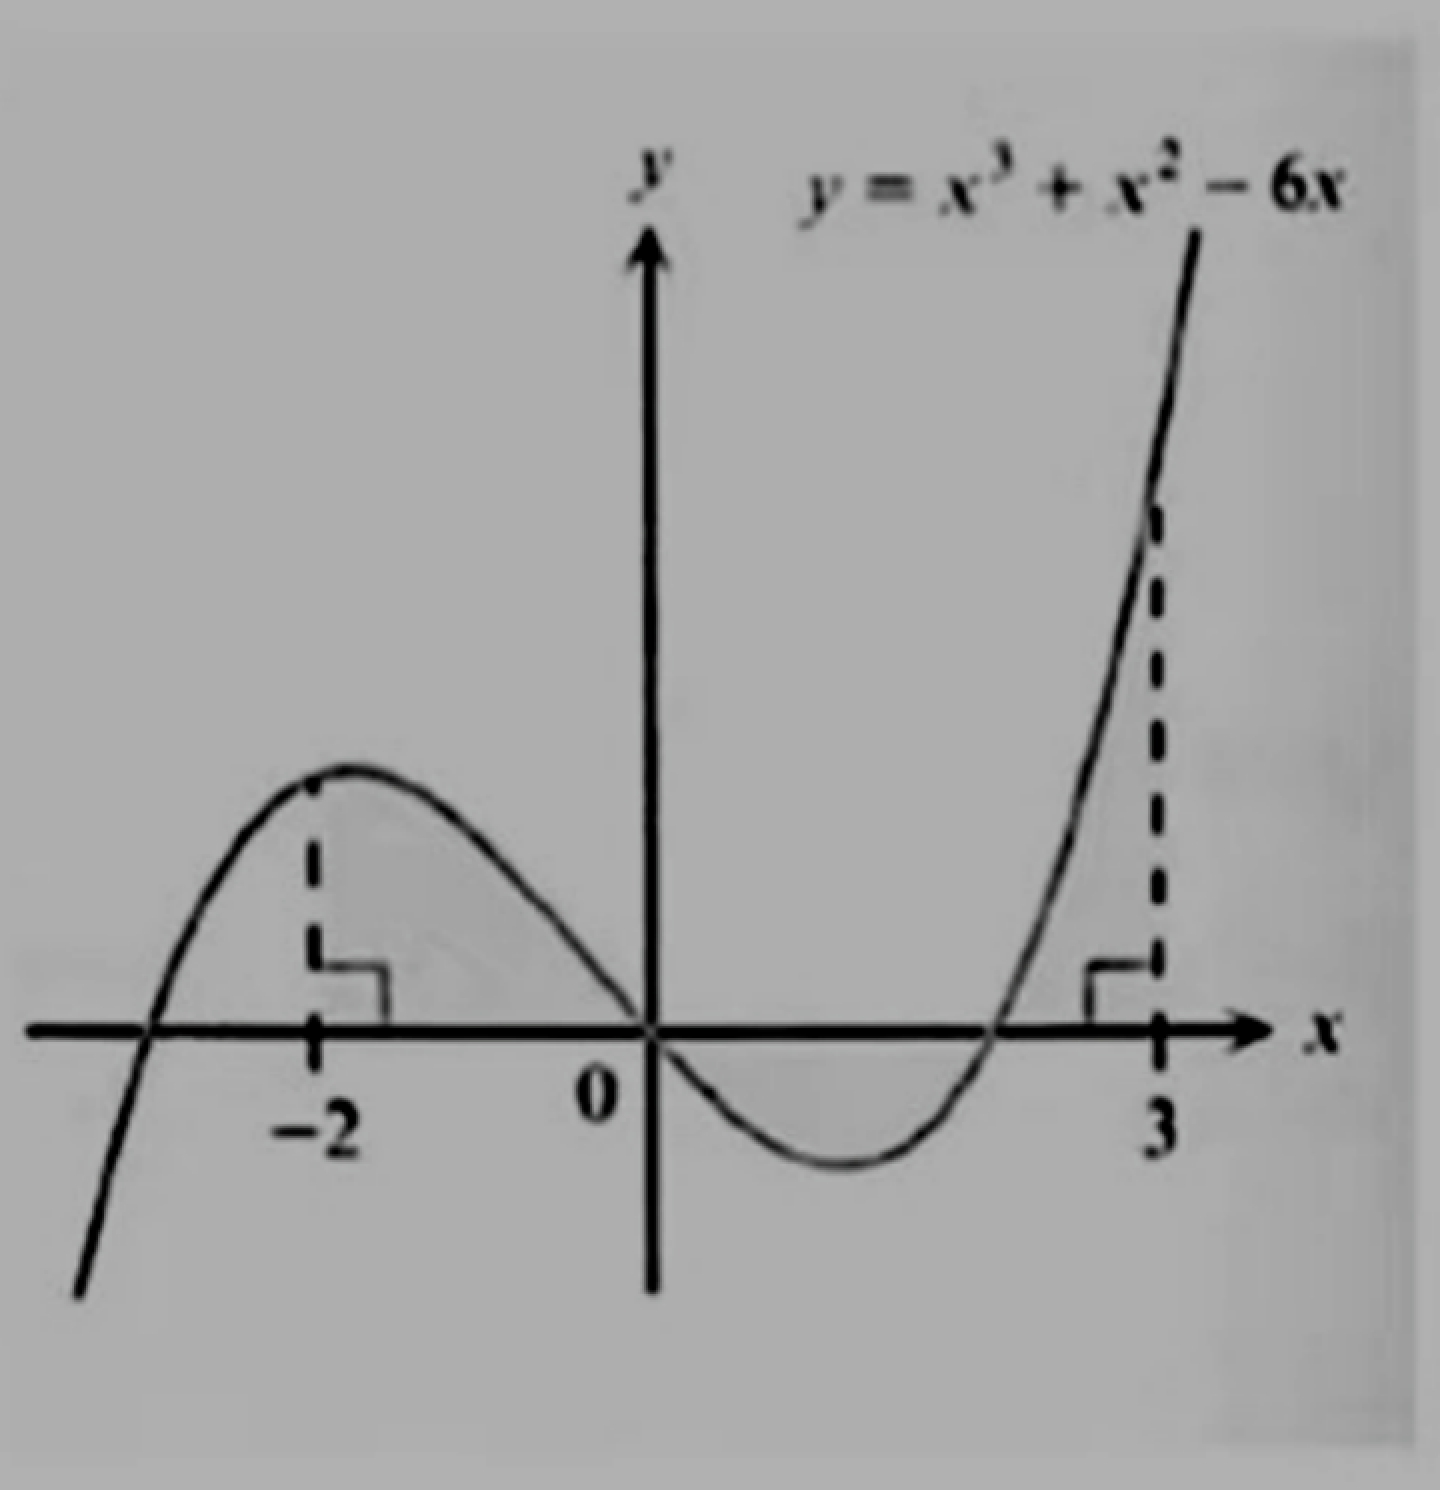
\includegraphics[width=5cm, height=3cm]{graph1.jpg}

\vspace{8\baselineskip}

\noindent \textbf{(10 marks)} Find the second derivative for each of the following functions with respect to $x$.\\
\indent (a) $y=\sqrt{2x+1}$\\
\indent (b) $e^{x^2}$





\section{Probability Theory}



\section{IQ}



\end{document}